\documentclass[12pt,a4paper,notitlepage,twoside,headsepline]{scrartcl}
\usepackage{pstool}
\usepackage{booktabs}
\usepackage[T1]{fontenc}
%\usepackage[latin1]{inputenc}
\usepackage{amsmath, amssymb, amsthm}
\usepackage{scrpage2}
\usepackage{lmodern}
\usepackage{microtype}
\usepackage[english]{babel}
% \usepackage{hyperref}
%%%%%%%%%%%%%%%%%%%%%%%%%%%%%%%%%%%%%%%%%%%%%%%%%%%%%%%%%%%%%%%%%%%%%%%%%%%%%%%
\def\ve#1{{\mathchoice{\mbox{\boldmath$\displaystyle #1$}}%
              {\mbox{\boldmath$\textstyle #1$}}%
              {\mbox{\boldmath$\scriptstyle #1$}}%
              {\mbox{\boldmath$\scriptscriptstyle #1$}}}}

%%%% Laengen %%%%%%%%%%%%%%%%%%%%%%%%%%%%%%%%%%%%%%%%%%%%%%%%%%%%%%%%%%%%%%%%%%
\unitlength1cm
\setcounter{secnumdepth}{5}
\setcounter{tocdepth}{5}
\textwidth=17cm
\textheight=23.5cm
\hoffset=-20mm
%\voffset=-10mm
\parindent0cm
\parskip.5em plus.1em minus .2em
\headheight6mm
\headsep8mm
\footskip22mm
\oddsidemargin16.0mm
\evensidemargin11.5mm
\renewcommand{\baselinestretch}{1.1}

%%%%%%%%%%%%%%%%%%%%%%%%%%%%%%%%%%%%%%%%%%%%%%%%%%%%%%%%%%%%%%%%%%%%%%%%%%%%%%%
% commands
\newcommand{\R}{\mathbb{R}}
\newcommand{\Z}{\mathbb{Z}}
\newcommand{\N}{\mathbb{N}}
\newcommand{\C}{\mathbb{C}}
\newcommand{\Q}{\mathbb{Q}}
\newcommand{\F}{\mathbb{F}}

%%%%%%%%%%%%%%%%%%%%%%%%%%%%%%%%%%%%%%%%%%%%%%%%%%%%%%%%%%%%%%%%%%%%%%%%%%%%%%%


%%%%%%%%%%%%%%%%%%%%%%%%%%%%%%%%%%%%%%%%%%%%
% Pagestyle
\pagestyle{scrheadings}
\clearscrheadfoot
\ihead{Document Title}	% Add the title of the document here.
\ohead{\pagemark}
%%%%%%%%%%%%%%%%%%%%%%%%%%%%%%%%%%%%%%%%%%%%
\EndPreamble % required by \pstool

% Begin of document
\begin{document}

\begin{titlepage}
\title{
\begin{center}
    {\Large\bfseries Seminar}   \\                
    {\large Special Topics on Communications, Winter Term 2012/2013}   \\[0.5cm]
    {\LARGE\bfseries Relaying and its Applications to LTE-Advanced}   \\[0.3cm] 
    \LaTeX\ example for seminar reports the Institute for Digital Communications (IDC)
\end{center}
}
\author{John Doe}
\date{October 15, 2009}
\end{titlepage}

%%%%%%%%%%%%%%%%%%%%%%%%%%%%%%%%%%%%%%%%%%%%
\maketitle

\begin{abstract}
\section*{Abstract}
An abstract contains a brief summary of a written document. It should fulfill the purpose of informing the reader of the paper's purpose and key findings.
\end{abstract}

%%%%%%%%%%%%%%%%%%%%%%%%%%%%%%%%%%%%%%%%%%%%
\section{Introduction}

We begin with the introduction by using the 
\verb|\section{Introduction}| command.


%%%%%%%%%%%%%%%%%%%%%%%%%%%%%%%%%%%%%%%%%%%%
\section{Generalities}

We continue with the next section using \verb|\section{Generalities}|. For an in-depth introduction to \LaTeX\ please refer to e.g. ~\cite{Kopka:1} (German book) or ~\cite{IntroLateX:08} (English PDF document).

If you need German "Umlaute" then please generate them with the following commmands: \verb|{\"a}|, \verb|{\"A}|, \verb|{\"o}|, \verb|{\"O}|, \verb|{\"u}|, \verb|{\"U}|. The German "{\ss}" can be generated by using the command \verb|{\ss}|.

All required (additional) packets have to be included by using the \verb|\usepackage{}| command at the beginning of the \LaTeX\ File. Please make sure to include standard packets only, such that the global layout and appearance remain unaltered.

%%%%%%%%%%%%%%%%%%%%%%%%%%%%%%%%%%%%%%%%%%%%
\section{Special Issues}

%%%%%%%%%%%%%%%%%%%%%%%%%%%%%%%%%%%%%%%%%%%%
\subsection{Mathematical Expressions and Equations}

Mathematical expressions and equations should be generated as e.g. stated in \cite[Kapitel 5]{Kopka:1}. 

The following equation is given by
\begin{equation}
\label{eq:equation_01}
   a = \frac{b}{c}\;,	% please consider equations as part of a sentence!
\end{equation}
and can be be referenced by \eqref{eq:equation_01}.

This paragraph was generated using the following \LaTeX\ source code:
\begin{verbatim}
The following equation is given by
\begin{equation}
\label{eq:equation_01}
   a = \frac{b}{c}\;,	% please treat equations as part of the sentence!
\end{equation}
and can be be referenced by \eqref{eq:equation_01}.
\end{verbatim}

Please use unambiguous labels!

In the template, some commands such as \verb|\R|, \verb|\Z|, \verb|\N|, \verb|\C|, and \verb|\Q| have already been defined. These commands generate the set symbols $\R$, $\Z$, $\N$, $\C$, and $\Q$, when the \LaTeX\ math mode is used. For  e.g. finite fields the symbol is $\F$ (generated by \verb+\F+) is provided. These predefined commands should be used.

In order to avoid confusing scalar, vector, or matrix variables, please stick to the following, well established rules:
\begin{itemize}
	\item Functions and other text are represented using a ``roman'' font. The corresponding 			command is \verb|\textrm{...}|.
	\item Scalar variables are represented using an ``italic'' font, which is the standard font for 			the \LaTeX\ math environment.
	\item Vectors should be represented by small, bold print italic letters. To this end, the command 
	\verb|\ve{...}| has been predefined.
	\item Matrices should be represented by capital, bold print italic letters. Again, the \verb|\ve{...}|
	command should be used to generate such symbols.
\end{itemize}

A further equation illustrating the Froebenius--Norm of an $M\times N$--dimensional matrix $\ve{A}$ is given by
\def\defeq{\stackrel{\mbox{\footnotesize def}}{=}}	
\begin{align}\label{eq:equation_02}
\|\ve{A}\|_{\mathrm{F}}^2 &\defeq  \sum_{m=1}^M \sum_{n=1}^N |a_{m,n}|^2 \;,\nonumber \\
&= \mathrm{spur}\left( \ve{A}\ve{A}^\mathsf{H} \right) \;.
\end{align}
This equation was generated using
\begin{verbatim}
% at first, we define the equation symbol with def on top
\def\defeq{\stackrel{\mbox{\footnotesize def}}{=}}	
% then we state the equation
\begin{align}\label{eq:equation_02}
\|\ve{A}\|_{\mathrm{F}}^2 
&\defeq \sum_{m=1}^M \sum_{n=1}^N |a_{m,n}|^2 \;,	\nonumber \\
&= \mathrm{spur}\left( \ve{A}\ve{A}^\mathsf{H} \right) \;.
\end{align}
\end{verbatim}

The \verb+\nonumber+ command suppresses the equation number in the first line of \eqref{eq:equation_02}.

%%%%%%%%%%%%%%%%%%%%%%%%%%%%%%%%%%%%%%%%%%%%%%%%%%%%%%%%%%%%%%%%%%%%%%%%%%%%%%%
\subsection{Figures}

Figures should be generated as .pdf files, and included into the document by employing the \verb+\includegraphics+ command.
Each figure should be combined with a concise caption, describing the figure's contents.
A typical example of a figure in a floating environment (used in pdfLaTeX) is generated by the following code:
\begin{verbatim}
\begin{figure}[!ht]
\begin{center}
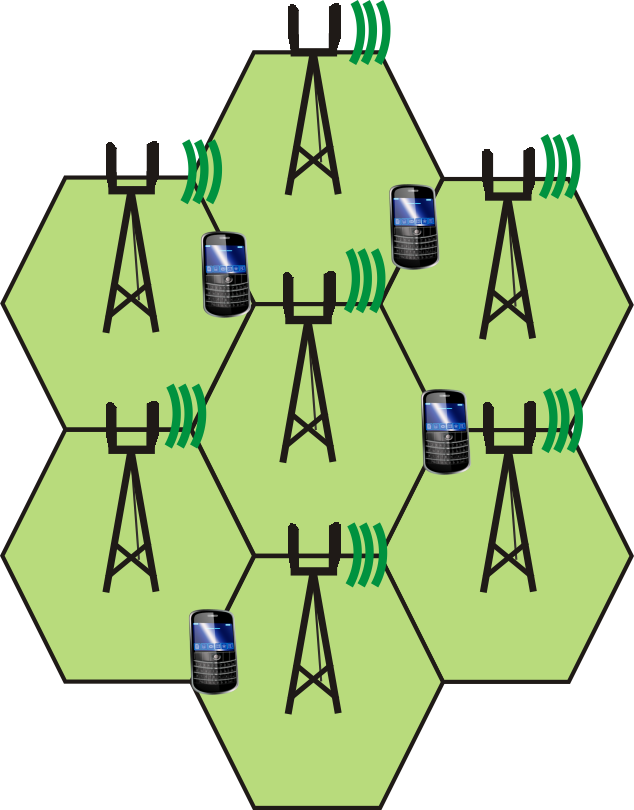
\includegraphics[width=0.25\textwidth]{figures/example}
\end{center}
\caption{This is an example figure according to \cite{Example09}.}
\label{fig:example}
\end{figure}
\end{verbatim}
% Here is the figure input
\begin{figure}[!ht]
\begin{center}
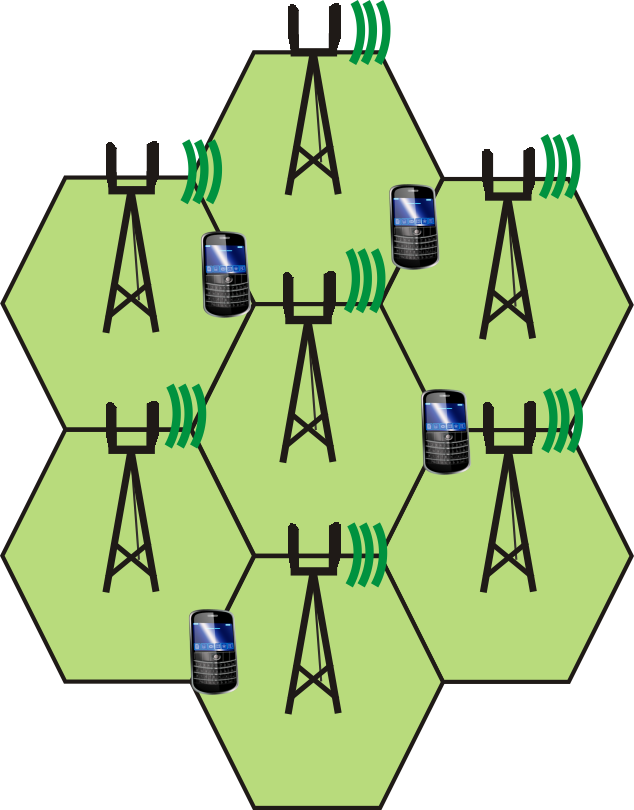
\includegraphics[width=0.25\textwidth]{figures/example}
\end{center}
\caption{This is an example figure according to \cite{Example09}.}
\label{fig:example}
\end{figure}

It is often desirable to replace sequences of letters from the original figure source file by other, possibly more appropriate abbreviations, words, or symbols. This can be achieved by using the  \verb+\pstool+ environment, which has been employed for generating Fig.~\ref{fig:example2}.  The \verb+\pstool+ environment converts an .eps (!) file (here: example2.eps) into a .pdf file, which is included in the final document. 

In this example, the letters \emph{U} and \emph{M}, as well as the German word \emph{Mobiltelefone} have been replaced by more fitting descriptions. As a prerequisite, all text symbols have to be embedded as text in the original figure .eps file. 

Fig.~\ref{fig:example2} has been generated with the following code:
\begin{figure}
    \begin{center}
    \pstool*[width=0.5\textwidth]{figures/example2}{
         \psfrag{U}[l][l]{Unicast cells}
    \psfrag{M}[l][l]{Multicast cells}
    \psfrag{Mobiltelefone}[l][l]{UEs}
         }
    \caption{An example for using the \textrm{pstool} environment.}
    \label{fig:example2}
    \end{center}
\end{figure}
\begin{verbatim}
\begin{figure}[htb]
\begin{center}
\pstool*[width=0.5\textwidth]{figures/example2}{
  \psfrag{U}[l][l]{Unicast cells}
  \psfrag{M}[l][l]{Multicast cells}
  \psfrag{Mobiltelefone}[l][l]{UEs}
}
\caption{An example for using the \textrm{pstool} environment.}
\label{fig:example2}
\end{center}
\end{figure}
\end{verbatim}

%%%%%%%%%%%%%%%%%%%%%%%%%%%%%%%%%%%%%%%%%%%%%%%%%%%%%%%%%%%%%%%%%%%%%%%%%%%%%%%
\subsection{Tables}
Tables are often required to provide a collective overview of used or generated data, such as e.g. a table illustrating simulation parameters. The following table is referenced by Tab.~\ref{tab:Table_01} and uses the table (floating) environment in combination with the tabular environment.
\begin{table}[htb]
\caption{A table example.}\label{tab:Table_01}
\centering\begin{tabular}{ll} \toprule
	Parameter    & Values \\
	\midrule
	Parameter 1 & value 1 \\
	Parameter 2 & Value 2 \\ \bottomrule
\end{tabular}
\end{table}

%%%%%%%%%%%%%%%%%%%%%%%%%%%%%%%%%%%%%%%%%%%%%%%%%%%%%%%%%%%%%%%%%%%%%%%%%%%%%%%
\subsection{The List of References}
At the end of this article, a list of references has to be included. This can achieved by either using
\begin{verbatim}
\begin{thebibliography}{whatever you want to write here}
\bibitem[Fis07]{Fischer:07}
R.\ Fischer: \emph{seminar.tex}, LIT, Uni Erlangen, Juli 2007.
\end{thebibliography}
\end{verbatim}
or
\begin{verbatim}
\bibliography{mein_bib_file}
\bibliographystyle{alpha}
\end{verbatim}
References to literature in the text are included by the \verb|\cite{...}| command. For example, the command
\verb|\cite{Fischer:07q}| would result in [Fis07].

%%%%%%%%%%%%%%%%%%%%%%%%%%%%%%%%%%%%%%%%%%%%%%%%%%%%%%%%%%%%%%%%%%%%%%%%%%%%%%%
\section{Conclusions}
Your article should not be missing a final statement containing some conclusions which can be drawn from your work. A reference to e.g. future work is also in order.

\iffalse
%%%%%%%%%%%%%%%%%%%%%%%%%%%%%%%%%%%%%%%%%%%%%%%%%%%%%%%%%%%%%%%%%%%%%%%%%%%%%%%
\section{Just another section.}

This is some more text.
This is some more text.
This is some more text.
This is some more text.
This is some more text.
This is some more text.
This is some more text.
This is some more text.
This is some more text.
This is some more text.
This is some more text.


\fi
%%%%%%%%%%%%%%%%%%%%%%%%%%%%%%%%%%%%%%%%%%%%%%%%%%%%%%%%%%%%%%%%%%%%%%%%%%%%%%%
\begin{thebibliography}{my bib}

\bibitem[Kop96]{Kopka:1}
H.\ Kopka: {\em \LaTeX\, Band I --- Einf{\"u}hrung}, 2.\ {\"u}berarbeitete Auflage,
    Addison--Wesley, 1996.
    
\bibitem[Oet08]{IntroLateX:08}
T.~Oetiker, H.~Partl, I.~Hyna and E.~Schlegl: The Not So Short Introduction to \LaTeX, available online
URL: http://www.ctan.org/tex-archive/info/lshort/english/lshort.pdf    

\bibitem[Exa09]{Example09}
F.\ Example: {\em Example Source}, Example Publisher, 2009.

\end{thebibliography}



%%%%%%%%%%%%%%%%%%%%%%%%%%%%%%%%%%%%%%%%%%%%%%%%%%%%%%%%%%%%%%%%%%%%%%%%%%%%%%%
\end{document}
